%%%%%%%%%%%%%%%%%%%%%%%%%%%%%%%%%%%%%%%%%%%%%%%%%%%%%%%%%%%%%%%%%%%%%%%%
%%%%%%%%%%%%%%%%%%%%%% Simple LaTeX CV Template %%%%%%%%%%%%%%%%%%%%%%%%
%%%%%%%%%%%%%%%%%%%%%%%%%%%%%%%%%%%%%%%%%%%%%%%%%%%%%%%%%%%%%%%%%%%%%%%%

%%%%%%%%%%%%%%%%%%%%%%%%%%%%%%%%%%%%%%%%%%%%%%%%%%%%%%%%%%%%%%%%%%%%%%%%
%% NOTE: If you find that it says                                     %%
%%                                                                    %%
%%                           1 of ??                                  %%
%%                                                                    %%
%% at the bottom of your first page, this means that the AUX file     %%
%% was not available when you ran LaTeX on this source. Simply RERUN  %%
%% LaTeX to get the ``??'' replaced with the number of the last page  %%
%% of the document. The AUX file will be generated on the first run   %%
%% of LaTeX and used on the second run to fill in all of the          %%
%% references.                                                        %%
%%%%%%%%%%%%%%%%%%%%%%%%%%%%%%%%%%%%%%%%%%%%%%%%%%%%%%%%%%%%%%%%%%%%%%%%

%%%%%%%%%%%%%%%%%%%%%%%%%%%% Document Setup %%%%%%%%%%%%%%%%%%%%%%%%%%%%

% Don't like 10pt? Try 11pt or 12pt
\documentclass[10pt]{article}
\usepackage[UTF8]{ctex}
% This is a helpful package that puts math inside length specifications
\usepackage{calc}
\usepackage{pifont}
\usepackage{marvosym}
\usepackage{graphicx}
\usepackage{wrapfig}
%\usepackage{verbatim} 


% Simpler bibsection for CV sections
% (thanks to natbib for inspiration)
\makeatletter
\newlength{\bibhang}
\setlength{\bibhang}{1em}
\newlength{\bibsep}
 {\@listi \global\bibsep\itemsep \global\advance\bibsep by\parsep}
\newenvironment{bibsection}%
        {\vspace{-\baselineskip}\begin{list}{}{%
       \setlength{\leftmargin}{\bibhang}%
       \setlength{\itemindent}{-\leftmargin}%
       \setlength{\itemsep}{\bibsep}%
       \setlength{\parsep}{\z@}%
        \setlength{\partopsep}{0pt}%
        \setlength{\topsep}{0pt}}}
        {\end{list}\vspace{-.6\baselineskip}}
\makeatother


% Layout: Puts the section titles on left side of page
\reversemarginpar

%
%         PAPER SIZE, PAGE NUMBER, AND DOCUMENT LAYOUT NOTES:
%
% The next \usepackage line changes the layout for CV style section
% headings as marginal notes. It also sets up the paper size as either
% letter or A4. By default, letter was used. If A4 paper is desired,
% comment out the letterpaper lines and uncomment the a4paper lines.
%
% As you can see, the margin widths and section title widths can be
% easily adjusted.
%
% ALSO: Notice that the includefoot option can be commented OUT in order
% to put the PAGE NUMBER *IN* the bottom margin. This will make the
% effective text area larger.
%
% IF YOU WISH TO REMOVE THE ``of LASTPAGE'' next to each page number,
% see the note about the +LP and -LP lines below. Comment out the +LP
% and uncomment the -LP.
%
% IF YOU WISH TO REMOVE PAGE NUMBERS, be sure that the includefoot line
% is uncommented and ALSO uncomment the \pagestyle{empty} a few lines
% below.
%

%% Use these lines for letter-sized paper
%\usepackage[paper=letterpaper,
%           %includefoot, % Uncomment to put page number above margin
%            marginparwidth=0.7in,     % Length of section titles
%            marginparsep=.05in,       % Space between titles and text
%            margin=0.5in,               % 1 inch margins
%            includemp]{geometry}

% Use these lines for A4-sized paper
\usepackage[paper=a4paper,
            %includefoot, % Uncomment to put page number above margin
            marginparwidth=24mm,    % Length of section titles
            marginparsep=1mm,       % Space between titles and text
            margin=15mm,              % 25mm margins
            includemp]{geometry}

%% More layout: Get rid of indenting throughout entire document
\setlength{\parindent}{0in}

%% This gives us fun enumeration environments. compactitem will be nice.
\usepackage{paralist}
\usepackage[shortlabels]{enumitem}


% \usepackage[misc]{ifsym}
%% Reference the last page in the page number
%
% NOTE: comment the +LP line and uncomment the -LP line to have a page
%       numbers without the ``of ##'' last page reference)
%
% NOTE: uncomment the \pagestyle{empty} line to get rid of all page
%       numbers (make sure include foot is commented out above)
%
\usepackage{fancyhdr,lastpage}
\pagestyle{fancy}
%\pagestyle{empty}      % Uncomment this to get rid of page numbers
\fancyhf{}\renewcommand{\headrulewidth}{0pt}
\fancyfootoffset{\marginparsep+\marginparwidth}
\newlength{\footpageshift}
\setlength{\footpageshift}
          {0.1\textwidth+0.1\marginparsep+0.1\marginparwidth-2in}
\lfoot{\hspace{\footpageshift}%
       \parbox{3.5in}{\, \hfill %
                    \arabic{page} of \protect\pageref*{LastPage} % +LP
%                    \arabic{page}                               % -LP
                    \hfill \,}}

% Finally, give us PDF bookmarks
\usepackage{color,hyperref}
\definecolor{darkblue}{rgb}{0.0,0.0,0.3}
\hypersetup{colorlinks,breaklinks,
            linkcolor=darkblue,urlcolor=darkblue,
            anchorcolor=darkblue,citecolor=darkblue}

%%%%%%%%%%%%%%%%%%%%%%%% End Document Setup %%%%%%%%%%%%%%%%%%%%%%%%%%%%


%%%%%%%%%%%%%%%%%%%%%%%%%%% Helper Commands %%%%%%%%%%%%%%%%%%%%%%%%%%%%

% The title (name) with a horizontal rule under it
%
% Usage: \makeheading{name}
%
% Place at top of document. It should be the first thing.
\newcommand{\makeheading}[1]%
        {\hspace*{-\marginparsep minus \marginparwidth}%
         \begin{minipage}[t]{\textwidth+\marginparwidth+\marginparsep}%
                {\large \bfseries #1}\\[-0.15\baselineskip]%
                 \rule{\columnwidth}{1pt}%
         \end{minipage}}

% The section headings
%
% Usage: \section{section name}
%
% Follow this section IMMEDIATELY with the first line of the section
% text. Do not put whitespace in between. That is, do this:
%
%       \section{My Information}
%       Here is my information.
%
% and NOT this:
%
%       \section{My Information}
%
%       Here is my information.
%
% Otherwise the top of the section header will not line up with the top
% of the section. Of course, using a single comment character (%) on
% empty lines allows for the function of the first example with the
% readability of the second example.
\renewcommand{\section}[2]%
        {\pagebreak[2]\vspace{1\baselineskip}%
         \phantomsection\addcontentsline{toc}{section}{#1}%
         \hspace{0in}%
         \marginpar{
         \raggedright \scshape #1}#2}

% An itemize-style list with lots of space between items
\newenvironment{outerlist}[1][\enskip\textbullet]%
        {%\begin{itemize}[#1]}{\end{itemize}%
        \begin{itemize}[label=#1, itemsep=1pt]}{\end{itemize}%%
         \vspace{-0.6\baselineskip}}

% An environment IDENTICAL to outerlist that has better pre-list spacing
% when used as the first thing in a \section
\newenvironment{lonelist}[1][\enskip\textbullet]%
        {\vspace{-\baselineskip}\begin{list}{#1}{%
        \setlength{\partopsep}{0pt}%
        \setlength{\topsep}{0pt}}}
        {\end{list}\vspace{-.6\baselineskip}}

% An itemize-style list with little space between items
% \newenvironment{innerlist}[1][\enskip\textbullet]%
\newenvironment{innerlist}[1][\enskip$\circ$]%
        {\begin{compactitem}[#1]}{\end{compactitem}}

% An environment IDENTICAL to innerlist that has better pre-list spacing
% when used as the first thing in a \section
\newenvironment{loneinnerlist}[1][\enskip\textbullet]%
        {\vspace{-\baselineskip}\begin{compactitem}[#1]}
        {\end{compactitem}\vspace{-.6\baselineskip}}

% To add some paragraph space between lines.
% This also tells LaTeX to preferably break a page on one of these gaps
% if a needed page break is nearby.
\newcommand{\blankline}{\quad\pagebreak[2]}

% Uses hyperref to link DOI
\newcommand\doilink[1]{\href{http://dx.doi.org/#1}{#1}}
\newcommand\doi[1]{doi:\doilink{#1}}


%%%%%%%%%%%%%%%%%%%%%%%% End Helper Commands %%%%%%%%%%%%%%%%%%%%%%%%%%%

%%%%%%%%%%%%%%%%%%%%%%%%% Begin CV Document %%%%%%%%%%%%%%%%%%%%%%%%%%%%

%\hyphenpenalty = 9999

\def\vs{\vspace{-0.1in}}
\begin{document}

% \makeheading{Curriculum Vitae\\ [0.3cm] TIEP HUU VU\quad~~~~~~\quad\quad\quad\quad\quad\quad\quad\quad\quad\quad\quad\quad\quad\quad{\small Last update: December 17, 2015}}



\newlength{\rcollength}\setlength{\rcollength}{3 in}
\vs

%% ==============================================================
\vspace{0.2in}

%\section{Research Background} % (fold)
%\label{sec:research_backg}
%\vspace{-0.25in}

%\begin{outerlist}
%  \item {\bf Graph Unsupervised Learning}: Graph Clustering/ Community Detection, Graph Representation Learning, Graph Contrastive Learning.
%  \item {\bf Graph Conformal Prediction:} Conformal Prediction for Node Classification.
%\end{outerlist}
% section research_backg (end)
%% =========  ==============================
	
% \makeheading{Curriculum Vitae\\ [0.3cm] TIEP HUU VU\quad~~~~~~\quad\quad\quad\quad\quad\quad\quad\quad\quad\quad\quad\quad\quad\quad{\small Last update: December 17, 2015}}
\makeheading{CHEN Han \hfill {\small Last update: Jan. 4, 2024}}

\vspace{-0.2in}
\section{contact\\information}
\begin{minipage}[l]{0.75\textwidth}
\begin{tabular}[t]{l@{}p{\textwidth-\rcollength}p{\rcollength}}
Tel: +86-13305014345\\
Tel: +65-89420214\\
{\large\Letter} \texttt{E-mail:}\href{mailto:concyclics@qq.com}{concyclics@qq.com} 
\\
{\large\Letter} \texttt{E-mail:}\href{mailto:chenhan@u.nus.edu}{chenhan@u.nus.edu} \\
\texttt{Github:}\href{https://www.github.com/Concyclics}{www.github.com/Concyclics}\\
\texttt{Linkedin:}\href{https://www.linkedin.com/in/han-chen-74784a233/}{linkedin.com/in/han-chen-74784a233}\\
%\texttt{Gitee:}\href{https://www.gitee.com/Concyclics}{www.gitee.com/concyclics}\\

%\texttt{Kaggle:}\href{https://www.kaggle.com/concyclics}{www.kaggle.com/concyclics} \\
\texttt{Address}: 09-01, West Coast Residental Village, 127371, Singapore\\												
\end{tabular}
\end{minipage}
\begin{minipage}[r]{0.5\textwidth}
\vspace{0.1in}
\quad \quad \quad \quad \quad \enspace 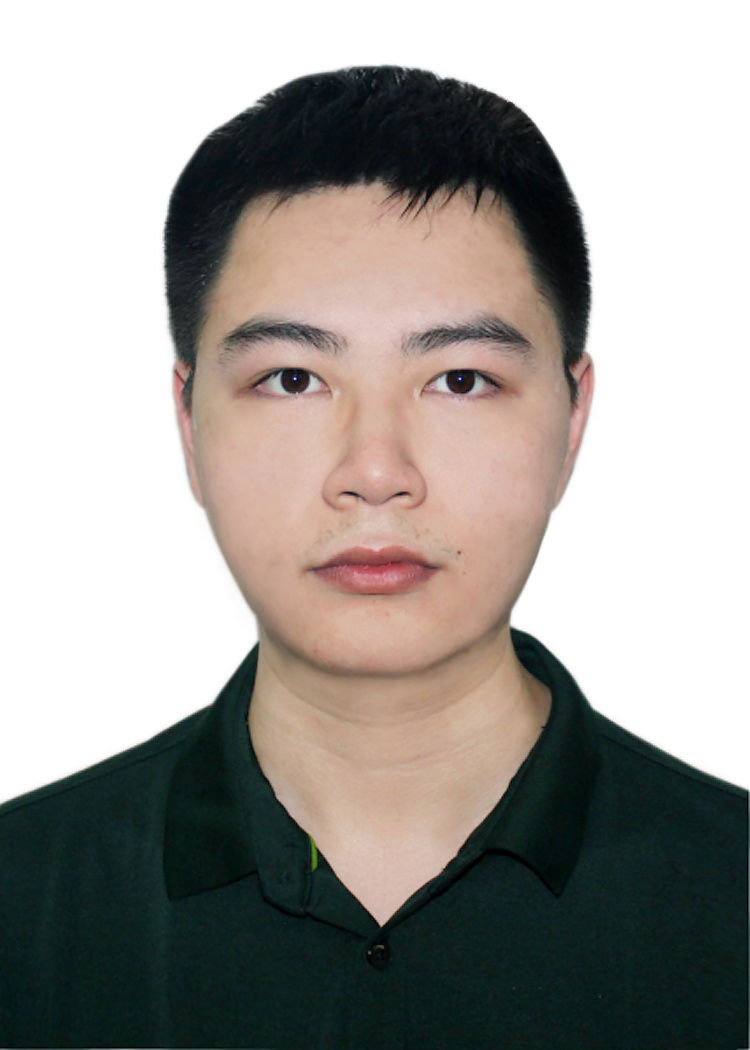
\includegraphics[width=0.25\textwidth]{face.jpg}\\
\end{minipage}
%% ==============================================================

%\section{Research Background} % (fold)
%\label{sec:research_backg}
%\vspace{-0.25in}

%\begin{outerlist}
%  \item {\bf Graph Unsupervised Learning}: Graph Clustering/ Community Detection, Graph Representation Learning, Graph Contrastive Learning.
%  \item {\bf Graph Conformal Prediction:} Conformal Prediction for Node Classification.
%\end{outerlist}
% section research_backg (end)
%% =========  ==============================
\noindent\rule{\textwidth}{1pt}
\section{education}
\vspace{-0.4in}

\href{https://www.nus.edu.sg/}{\textbf{National University of Singapore}}, Singapore. \hfill 2023--2025(Expected)
        \begin{innerlist}
                \item Master of Computing, Computer Science Specialization. \hfill GPA: 4.38/5.0
        \end{innerlist}

\href{https://www.scut.edu.cn/en/}{\textbf{South China University of Technology (SCUT)}}, Guangzhou, China. \hfill 2019--2023
\begin{innerlist}
        \item B.Eng., Software Engineering.\hfill GPA: 3.61/4.0
\end{innerlist}

%\href{http://www.fzsz.net/}{\textbf{Fuzhou NO.3 High School}}, Fuzhou, China. \hfill 2016--2019
  

%% =========  ==============================
\noindent\rule{\textwidth}{1pt}
\section{Honors \\and\\ Awards}
\vspace{-0.5in}
\begin{outerlist}

        \item \href{https://concyclics.github.io/resume/certificates/%E4%BC%98%E7%A7%80%E6%AF%95%E8%AE%BE%E8%AF%81%E4%B9%A6.pdf}
        {\textbf{Outstanding Dissertation of South China University of Technology}} \hfill 2023
        
        \item \href{https://concyclics.github.io/resume/certificates/%E6%95%B0%E6%A8%A1H%E5%A5%96.pdf}
        {\textbf{Honorable Mention} Mathematical Contest in Modeling} \hfill 2023

        \item \href{https://concyclics.github.io/resume/certificates/%E5%9B%BD%E5%A5%96%E8%AF%81%E4%B9%A6.pdf}
        {\textbf{National Scholarship}} \hfill 2022

	\item \href{https://concyclics.github.io/resume/certificates/ECfinal%E4%B8%AA%E4%BA%BA.pdf}
        {\textbf{\textit{Bronze Medal (46th)}} ICPC Asia-East Continent Final} \hfill 2022

	%\item \textbf{\textit{Silver Medal (3rd)}} \\National College Students Algorithm Design\&Programming Challenge Contest\hfill 2022

        \item \href{https://concyclics.github.io/resume/certificates/%E5%8C%BA%E5%9F%9F%E8%B5%9B%E9%93%B6%E7%89%8C.pdf}
        {\textbf{\textit{Silver Medal (46th)}} ICPC Asia JiNan Regional Contest} \hfill 2021

	
	%\item \textbf{\textit{The First Prize Scholarship} Hong Ping Evergreen Fund}\\Student Science and Technology Innovation Competition scholarship\hfill 2022

	%\item \textbf{\textit{Outstanding Contribution Award}} \\Extracurricular Academic Science and Technology Innovation\&Competition of 
	%\\South China University of Technology\hfill 2022
	
	%\item \textbf{\textit{Kaggle Dataset Expert}} \href{https://www.kaggle.com/concyclics}{Rank 181/63093} \hfill 2022

	%\item \textbf{\textit{Kaggle Notebook Expert}} \href{https://www.kaggle.com/concyclics}{Rank 964/221587} \hfill 2022
\end{outerlist}


%% ================== block:  ==========================
\noindent\rule{\textwidth}{1pt}
\section{Project and \\Internship\\Experience}
\vspace{-0.5in}
\begin{outerlist}

\item {\it\textbf{Symmetric Matrix Solving Algorithm Parallel Optimization for ARM Architecture}}\\
	Mentor: \href{http://www2.scut.edu.cn/sse/2018/0614/c16789a270678/page.htm}{Prof. Deyou TANG}\hfill May-Dec. 2022\\
	\vspace{-0.2in}
	\begin{innerlist}
		\item Implemente the subroutine of bounded Bunch-Kaufman algorithm and use openmp and NEON intrinsics to optimize parallelism and performance.
		\item Modify the cache-hit rate and parallelism during column-swap part to achieve a 70\% total performance improvement.
	\end{innerlist}

\item {\it\textbf{Research Assistant}} in \textbf{\href{https://hkust-gz.edu.cn/zh/?variant=zh-cn}{Hong Kong University of Science and Technology, Guangzhou}}\\
Mentor: \href{https://zeyiwen.github.io/}{Prof. Zeyi WEN}\hfill Apr-Sept.  2023\\
\vspace{-0.2in}
\begin{innerlist}
        \item Research on the Graph Partitioning Algorithm and fillin-reducing ordering algorithm.
        \item Use omp task to optimize and parallel the graph partitioning algorithm.
\end{innerlist}

\item {\it\textbf{Internship}} in \textbf{SG Digital Trust Lab, Singapore Research Center, 2012 Laboratory}\\
Mentor: Dr. Tao HUANG\hfill Jan.-May.  2024(Expected)\\
Topic1: High Performance Symmetric Encryption Algorithm\\
Topic2: Efficient Model Stealing Defence\\
\end{outerlist}

 %% =========  ==============================
 \noindent\rule{\textwidth}{1pt}

\section{Technical Skills} % (fold)
\vspace{-0.5in}
\begin{outerlist}
  	\item {\it English}: IELTS(6.5), CET-4, CET-6.
  	\item {\it familiar with}: C/C++, Fortran, p4-16, blas, openmp, mpi, pthread, cuda.
  	\item {\it TestDemo Certificate}: \href{https://app.testdome.com/cert/bc443ba08d3442d1a4de9e7aea611dfa}{C++, TOP 10\%}, \href{https://app.testdome.com/cert/71e9426611324cce8a5dff69d23da9a5}{LINUX, TOP 10\%}, \href{https://app.testdome.com/cert/9af88d532837416f80620799c6fa1c9f}{PYTHON, TOP 10\%}.
   	\item {\it Kaggle Certificate}: \href{https://www.kaggle.com/learn/certification/concyclics/data-visualization}{Data Visualization}, \href{https://www.kaggle.com/learn/certification/concyclics/intro-to-machine-learning}{Intro to Machine Learning}, \href{https://www.kaggle.com/learn/certification/concyclics/intro-to-deep-learning}{Intro to Deep Learning}, \href{https://www.kaggle.com/learn/certification/concyclics/intro-to-game-ai-and-reinforcement-learning}{Intro to Game AI and Reinforcement Learning}.
  %\item {\it Technical Softwares}: MATLAB.
\end{outerlist}

%% ================== block:  ==========================%
\noindent\rule{\textwidth}{1pt}
\section{Exchange\\Experience}
\vspace{-0.5in}
\begin{outerlist}
\item \textbf{Online Academic Program on Machine Learning, McGill University} \hfill Jan.-Feb. 2022\\
\end{outerlist}

% \makeheading{Curriculum Vitae\\ [0.3cm] TIEP HUU VU\quad~~~~~~\quad\quad\quad\quad\quad\quad\quad\quad\quad\quad\quad\quad\quad\quad{\small Last update: December 17, 2015}}


%% ==============================================================


%\section{Research Background} % (fold)
%\label{sec:research_backg}
%\vspace{-0.25in}

%\begin{outerlist}
%  \item {\bf Graph Unsupervised Learning}: Graph Clustering/ Community Detection, Graph Representation Learning, Graph Contrastive Learning.
%  \item {\bf Graph Conformal Prediction:} Conformal Prediction for Node Classification.
%\end{outerlist}
% section research_backg (end)
%% =========  ==============================
\pagebreak
	
% \makeheading{Curriculum Vitae\\ [0.3cm] TIEP HUU VU\quad~~~~~~\quad\quad\quad\quad\quad\quad\quad\quad\quad\quad\quad\quad\quad\quad{\small Last update: December 17, 2015}}
\makeheading{陈 涵 \hfill {\small 最近更新: 2024年1月4日}}


\vspace{-0.2in}
\section{联系方式}
\begin{minipage}[l]{0.75\textwidth}
\begin{tabular}[t]{l@{}p{\textwidth-\rcollength}p{\rcollength}}
Tel: +86-13305014345\\
Tel: +65-89420214\\
{\large\Letter} \texttt{E-mail:}\href{mailto:concyclics@qq.com}{concyclics@qq.com}\\
{\large\Letter} \texttt{E-mail:}\href{mailto:chenhan@u.nus.edu}{chenhan@u.nus.edu} \\
\texttt{Github:}\href{https://www.github.com/Concyclics}{www.github.com/Concyclics}\\
\texttt{领英:}\href{https://www.linkedin.com/in/han-chen-74784a233/}{linkedin.com/in/han-chen-74784a233}\\
%\texttt{Gitee:}\href{https://www.gitee.com/Concyclics}{www.gitee.com/concyclics}\\
%\texttt{Kaggle:}\href{https://www.kaggle.com/concyclics}{www.kaggle.com/concyclics} \\
\texttt{地址}: 新加坡 West Coast Residental Village 09-01 127371\\												
\end{tabular}
\end{minipage}
\begin{minipage}[r]{0.5\textwidth}
\vspace{0.1in}
\quad \quad \quad \quad \quad \enspace 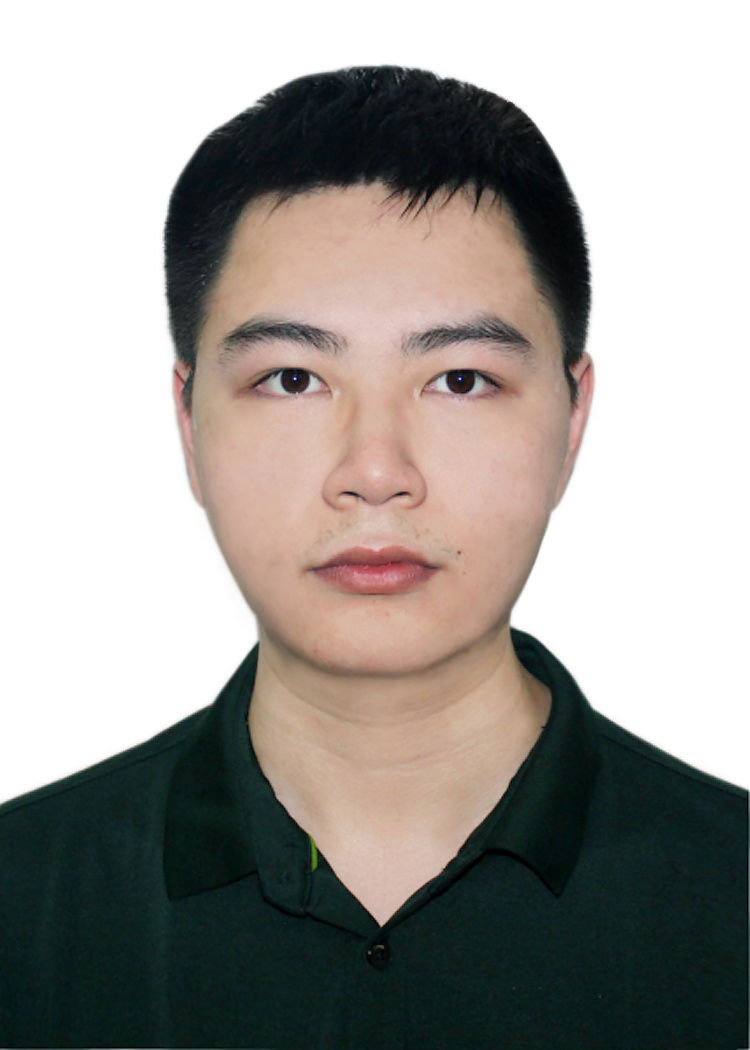
\includegraphics[width=0.25\textwidth]{face.jpg}\\
\end{minipage}

%% ==============================================================

%\section{Research Background} % (fold)
%\label{sec:research_backg}
%\vspace{-0.25in}

%\begin{outerlist}
%  \item {\bf Graph Unsupervised Learning}: Graph Clustering/ Community Detection, Graph Representation Learning, Graph Contrastive Learning.
%  \item {\bf Graph Conformal Prediction:} Conformal Prediction for Node Classification.
%\end{outerlist}
% section research_backg (end)
%% =========  ==============================
\noindent\rule{\textwidth}{1pt}
\section{教育经历}
\vspace{-0.4in}
\\
\href{https://www.nus.edu.sg/}{\textbf{新加坡国立大学}}, 新加坡 \hfill 2023--2025(预计)
\begin{innerlist}
        \item 计算机科学硕士, 计算机科学方向. \hfill GPA: 4.38/5.0
\end{innerlist}
\href{https://www.scut.edu.cn/en/}{\textbf{华南理工大学}}, 广东省广州市 \hfill 2019--2023
\begin{innerlist}
        \item 工学学士, 软件工程专业. \hfill GPA: 3.61/4.0
\end{innerlist}
%\href{http://www.fzsz.net/}{\textbf{福建省福州第三中学}}, 福建省福州市. \hfill 2016--2019




\noindent\rule{\textwidth}{1pt}
\section{获奖荣誉}
\vspace{-0.5in}
\begin{outerlist}

%\item 华南理工大学\textbf{\textit{优秀共青团员}} \hfill 2019\&2021
\item \href{https://concyclics.github.io/resume/certificates/%E4%BC%98%E7%A7%80%E6%AF%95%E8%AE%BE%E8%AF%81%E4%B9%A6.pdf}
{\textbf{华南理工大学本科优秀毕业设计(论文)}} \hfill 2023
\item \href{https://concyclics.github.io/resume/certificates/%E6%95%B0%E6%A8%A1H%E5%A5%96.pdf}
{\textbf{二等奖} 美国大学生数学建模竞赛 (MCM/ICM)} \hfill 2023

\item \href{https://concyclics.github.io/resume/certificates/ECfinal%E4%B8%AA%E4%BA%BA.pdf}
{\textbf{\textit{铜牌}} 第46届ICPC国际大学生程序设计竞赛亚洲区决赛} \hfill 2022
\item \href{https://concyclics.github.io/resume/certificates/%E5%9B%BD%E5%A5%96%E8%AF%81%E4%B9%A6.pdf}
{\textbf{国家奖学金}} \hfill 2022

\item \href{https://concyclics.github.io/resume/certificates/%E5%8C%BA%E5%9F%9F%E8%B5%9B%E9%93%B6%E7%89%8C.pdf}
{\textbf{\textit{银牌}} 第46届ICPC国际大学生程序设计竞赛(济南站)} \hfill 2021
%\item \textbf{\textit{顽强拼搏奖}} 第46届国际大学生程序设计竞赛亚洲区决赛 \hfill 2022
%\item \textbf{\textit{银牌}} 第三届全国大学生算法设计与编程挑战赛 (秋季赛) \hfill 2022
%\item \textbf{\textit{铜牌}} 第三届全国大学生算法设计与编程挑战赛 (冬季赛) \hfill 2022
%\item \textbf{\textit{铜牌}} 第三届全国大学生算法设计与编程挑战赛 (夏季赛) \hfill 2022
%\item \textbf{\textit{一等奖}} “宏平长青基金”学生科技创新竞赛奖学金\hfill 2022
%\item  \textbf{\textit{银牌}} 集美大学第八届程序设计竞赛. \hfill 2022
%\item \textbf{\textit{杰出贡献奖}} 华南理工大学课外学术科技创新竞赛成果\hfill 2022
%\item \textbf{\textit{Kaggle 数据专家(Dataset Expert)}} \href{https://www.kaggle.com/concyclics}{排名 181/63093} \hfill 2022
%\item \textbf{\textit{Kaggle 代码专家(Notebook Expert)}} \href{https://www.kaggle.com/concyclics}{排名 964/221587} \hfill 2022
\end{outerlist}
\noindent\rule{\textwidth}{1pt}

%% ================== block:  ==========================
\vspace{0.1in}

%% ================== block:  ==========================
\section{项目和实习\\经历} % (fold)
\label{sec:technical_ski}
\vspace{-0.5in}
\begin{outerlist}
 	
 \item {\it \textbf{对称矩阵函数求解BBK算法的并行优化}} \hfill 2022/04-2022/12\\
 	单位:  	华为鲲鹏计算\quad
 	导师: \href{http://www2.scut.edu.cn/sse/2018/0614/c16789a270678/page.htm}{汤德佑教授}
        \begin{innerlist}
                \item 实现Bounded Bunch-Kaufman (BBK)算法,利用NEON指令集和OpenMP进行优化。
                \item 对求解的行交换操作进行并行和访存局部性优化,实现总体接口70\%的性能提升。
        \end{innerlist}

 \item {\it\textbf{科研助理}} \hfill 2023/04--2023/09\\
        单位: \href{https://hkust-gz.edu.cn/zh/?variant=zh-cn}{香港科技大学广州校区}\quad
        导师: \href{https://zeyiwen.github.io/}{文泽忆教授}
        \begin{innerlist}
                %\item Research on the Graph Partitioning Algorithm and fillin-reducing ordering algorithm.
                \item 开展图分割算法和填充减少排序算法的研究。
                \item 利用omp task对图分割算法进行并行优化。
        \end{innerlist}

 \item {\it\textbf{实习生}} \hfill 2024/01--2024/05(预计)\\
        单位: 华为2012实验室亚太研究院新加坡研究所数字信任实验室\\
        导师:黄涛博士\\
        项目1: 高性能对称加密算法\\
        项目2: 高效的模型窃取防御\\
        
\end{outerlist}
%% =========  ==============================
\noindent\rule{\textwidth}{1pt}
\section{专业技能} % (fold)
\label{sec:technical_ski}
\vspace{-0.5in}
\begin{outerlist}
  \item {\it 英语认证水平}: CET-4, CET-6, IELTS(6.5). 
  \item {\it 编程技能}: C/C++, Fortran, p4-16, blas, openmp, mpi, pthread, cuda. 
  \item {\it TestDemo 编程技能认证}: \href{https://app.testdome.com/cert/bc443ba08d3442d1a4de9e7aea611dfa}{C++, TOP 10\%}, \href{https://app.testdome.com/cert/71e9426611324cce8a5dff69d23da9a5}{LINUX, TOP 10\%}, \href{https://app.testdome.com/cert/9af88d532837416f80620799c6fa1c9f}{PYTHON, TOP 10\%}
\item {\it Kaggle 课程认证}: \href{https://www.kaggle.com/learn/certification/concyclics/data-visualization}{数据可视化}, \href{https://www.kaggle.com/learn/certification/concyclics/intro-to-machine-learning}{机器学习}, \href{https://www.kaggle.com/learn/certification/concyclics/intro-to-deep-learning}{深度学习}, \href{https://www.kaggle.com/learn/certification/concyclics/intro-to-game-ai-and-reinforcement-learning}{强化学习}

\end{outerlist}

\noindent\rule{\textwidth}{1pt}
\section{交换经历}
\vspace{-0.5in}
\begin{outerlist}
\item \textbf{机器学习线上访学项目, 麦吉尔大学} \hfill 2022/01--2022/02\\
\end{outerlist}

%% ================== block:  ==========================%

\end{document}